 \documentclass{article}
\usepackage{graphicx} % Required for inserting images
% header

%% natbib
\usepackage{natbib}
\bibliographystyle{plain}

%% comment
\usepackage{comment}

% no automatic indentation
\usepackage{indentfirst}

% manually indent
\usepackage{xargs} % \newcommandx
\usepackage{calc} % calculation
\newcommandx{\tab}[1][1=1]{\hspace{\fpeval{#1 * 10}pt}}
% \newcommand[number of parameters]{output}
% \newcommandx[number of parameters][parameter index = x]{output}
% use parameter index = x to substitute the default argument
% use #1, #2, ... to get the first, second, ... arguments
% \tab for indentation
% \tab{2} for for indentation twice

% note
\newcommandx{\note}[1]{\textit{\textcolor{red}{#1}}}
\newcommand{\todo}{\note{TODO}}
% \note{TODO}

%% math package
\usepackage{amsfonts}
\usepackage{amsmath}
\usepackage{amssymb}
\usepackage{tikz-cd}
\usepackage{mathtools}
\usepackage{amsthm}

%% operator
\DeclareMathOperator{\tr}{tr}
\DeclareMathOperator{\diag}{diag}
\DeclareMathOperator{\sign}{sign}
\DeclareMathOperator{\grad}{grad}
\DeclareMathOperator{\curl}{curl}
\DeclareMathOperator{\Div}{div}
\DeclareMathOperator{\card}{card}
\DeclareMathOperator{\Span}{span}
\DeclareMathOperator{\real}{Re}
\DeclareMathOperator{\imag}{Im}
\DeclareMathOperator{\supp}{supp}
\DeclareMathOperator{\im}{im}
\DeclareMathOperator{\aut}{Aut}
\DeclareMathOperator{\inn}{Inn}
\DeclareMathOperator{\Char}{char}
\DeclareMathOperator{\Sylow}{Syl}
\DeclareMathOperator{\coker}{coker}
\DeclareMathOperator{\inc}{in}
\DeclareMathOperator{\Sd}{Sd}
\DeclareMathOperator{\Hom}{Hom}
\DeclareMathOperator{\interior}{int}
\DeclareMathOperator{\ob}{ob}
\DeclareMathOperator{\Set}{Set}
\DeclareMathOperator{\Top}{Top}
\DeclareMathOperator{\Meas}{Meas}
\DeclareMathOperator{\Grp}{Grp}
\DeclareMathOperator{\Ab}{Ab}
\DeclareMathOperator{\Ch}{Ch}
\DeclareMathOperator{\Fun}{Fun}
\DeclareMathOperator{\Gr}{Gr}
\DeclareMathOperator{\End}{End}
\DeclareMathOperator{\Ad}{Ad}
\DeclareMathOperator{\ad}{ad}
\DeclareMathOperator{\Bil}{Bil}
\DeclareMathOperator{\Skew}{Skew}
\DeclareMathOperator{\Tor}{Tor}
\DeclareMathOperator{\Ho}{Ho}
\DeclareMathOperator{\RMod}{R-Mod}
\DeclareMathOperator{\Ev}{Ev}
\DeclareMathOperator{\Nat}{Nat}
\DeclareMathOperator{\id}{id}
\DeclareMathOperator{\Var}{Var}
\DeclareMathOperator{\Cov}{Cov}
\DeclareMathOperator{\RV}{RV}
\DeclareMathOperator{\rank}{rank}

%% pair delimiter
\DeclarePairedDelimiter{\abs}{\lvert}{\rvert}
\DeclarePairedDelimiter{\inner}{\langle}{\rangle}
\DeclarePairedDelimiter{\tuple}{(}{)}
\DeclarePairedDelimiter{\bracket}{[}{]}
\DeclarePairedDelimiter{\set}{\{}{\}}
\DeclarePairedDelimiter{\norm}{\lVert}{\rVert}

%% theorems
\newtheorem{axiom}{Axiom}
\newtheorem{definition}{Definition}
\newtheorem{theorem}{Theorem}
\newtheorem{proposition}{Proposition}
\newtheorem{corollary}{Corollary}
\newtheorem{lemma}{Lemma}
\newtheorem{remark}{Remark}
\newtheorem{claim}{Claim}
\newtheorem{problem}{Problem}
\newtheorem{assumption}{Assumption}
\newtheorem{example}{Example}
\newtheorem{exercise}{Exercise}

%% empty set
\let\oldemptyset\emptyset
\let\emptyset\varnothing

\newcommand\eps{\epsilon}

% mathcal symbols
\newcommand\Tau{\mathcal{T}}
\newcommand\Ball{\mathcal{B}}
\newcommand\Sphere{\mathcal{S}}
\newcommand\bigO{\mathcal{O}}
\newcommand\Power{\mathcal{P}}
\newcommand\Str{\mathcal{S}}


% mathbb symbols
\usepackage{mathrsfs}
\newcommand\N{\mathbb{N}}
\newcommand\Z{\mathbb{Z}}
\newcommand\Q{\mathbb{Q}}
\newcommand\R{\mathbb{R}}
\newcommand\C{\mathbb{C}}
\newcommand\F{\mathbb{F}}
\newcommand\T{\mathbb{T}}
\newcommand\Exp{\mathbb{E}}

% mathrsfs symbols
\newcommand\Borel{\mathscr{B}}

% algorithm
\usepackage{algorithm}
\usepackage{algpseudocode}

% longproof
\newenvironment{longproof}[1][\proofname]{%
  \begin{proof}[#1]$ $\par\nobreak\ignorespaces
}{%
  \end{proof}
}


% for (i) enumerate
% \begin{enumerate}[label=(\roman*)]
%   \item First item
%   \item Second item
%   \item Third item
% \end{enumerate}
\usepackage{enumitem}

% insert url by \url{}
\usepackage{hyperref}

% margin
\usepackage{geometry}
\geometry{
a4paper,
total={190mm,257mm},
left=10mm,
top=20mm,
}


\title{ma5209 assignment 3}
\author{Nguyen Ngoc Khanh - A0275047B}
\date{March 2024}

\begin{document}
\maketitle

\section{Problem 1}

\begin{enumerate}[label=(\alph*)]
    \item Let $p$ be a prime number and let $\Z[1/p]$ be the subring of $\Q$ consisting of rational numbers whose denominators are powers of $p$. Construct compatible maps $\Z / p^n \Z \to \Z[1/p]/\Z$ and show that
    $$
        \varinjlim \Z / p^n \Z \xrightarrow{\cong} \Z[1/p]/\Z
    $$
    This is the "$p$-torsion Prüfer group"

    \item Show that $\Q / \Z \cong \bigoplus_p \Z_{p^\infty}$ where the direct sum runs over the prime numbers.

    \item Show that $\Tor_1(A, \Z_{p^\infty})$ and $\Tor_1(A, \Q / \Z)$ are naturally isomorphic to certain subgroups of $A$

    \item Compute $H_*(\R P^n; \Q / \Z)$
\end{enumerate}

\subsection{(a)}

\begin{center}
\begin{tikzcd}
0 \arrow[rr] &  & \Z / p^1 \Z \arrow[rr] &  & ... \arrow[rr] &  & \Z / p^{n-1} \Z \arrow[rr, "f_n"] \arrow[rrdd, "g_{n-1}"'] &  & \Z / p^n \Z \arrow[rr] \arrow[dd, "g_n"] &  & ... \\
             &  &                        &  &                &  &                                                            &  &                                          &  &     \\
             &  &                        &  &                &  &                                                            &  & {\Z[1/p]/\Z}                             &  &    
\end{tikzcd}
\end{center}

We define $f_n: \Z / p^{n-1} \Z \to \Z / p^n \Z$ and $g_n: \Z / p^n \Z \to \Z[1/p]/\Z$ as follows:

$$
    f_n: [a] \mapsto [pa]
$$

$$
    g_n: [a] \mapsto \bracket*{\frac{a}{p^n}}
$$

where $a \in \Z$. We will verify that $f_n, g_n$ are well-defined, group homomorphisms and $\Z[1/p]/\Z$ is the direct limit.

\begin{enumerate}
    \item $f_n$ is well-defined
    $$
        f_n([a + k p^{n-1}]) = [p(a + k p^{n-1})] = [pa + k p^n] = [pa] = f([a])
    $$

    \item $f_n$ is a homomorphism
    $$
        f_n([a] + [b]) = f_n([a + b]) = [p(a + b)] = [pa + pb] = [pa] + [pb] = f_n([a]) + f_n([b])
    $$

    \item $g_n$ is well-defined
    $$
        g_n([a + k p^n]) = \bracket*{\frac{a + k p^n}{p^n}} = \bracket*{\frac{a}{p^n} + k} = \bracket*{\frac{a}{p^n}} = g_n([a])
    $$

    \item $g_n$ is a homomorphism
    $$
        g_n([a] + [b]) = g_n([a + b]) = \bracket*{\frac{a + b}{p^n}} = \bracket*{\frac{a}{p^n} + \frac{b}{p^n}} = \bracket*{\frac{a}{p^n}} + \bracket*{\frac{b}{p^n}} = g_n([a]) + g_n([b])
    $$

    Note that $\bracket*{\frac{a}{p^n} + \frac{b}{p^n}} = \bracket*{\frac{a}{p^n}} + \bracket*{\frac{b}{p^n}}$ is due to $x$ and $x + 1$ identify the same element in $p$-torsion Prüfer group

    \item $g_{n-1} = g_n f_n$
    $$
        g_n(f_n([a])) = g_n([pa]) = \bracket*{\frac{pa}{p^n}} = \bracket*{\frac{a}{p^{n-1}}} = g_{n-1}([a])
    $$

    \item direct limit

    Note that each $f_n$ and $g_n$ is a monomorphism, we have the filtration
    $$
        0 \subseteq g_1(\Z / p^1 \Z) \subseteq ... \subseteq g_{n-1}(\Z / p^{n-1} \Z) \subseteq g_n(\Z / p^n \Z) \subseteq ... \subseteq \Z[1/p]/\Z
    $$
    and $\Z[1/p]/\Z = \bigcup_{n=0}^\infty g_n(\Z / p^n \Z)$ which is exactly the direct limit.
\end{enumerate}

\subsection{(b)}

Define an isomorphism $\alpha: \bigoplus_p \Z_{p^\infty} \to \Q / \Z$ as follows

$$
    \alpha: \tuple*{\bracket*{\frac{a_1}{p_1^{n_1}}}, \bracket*{\frac{a_2}{p_2^{n_2}}}, ...} \mapsto \bracket*{\sum_{i=1}^\infty \frac{a_i}{p_i^{n_i}}}
$$



We will prove that $\alpha$ is an isomorphism by verifying $\alpha$ is a bijective homomorphism

\begin{enumerate}
    \item $\alpha$ is an homomorphism

    $\alpha$ is a direct product of inclusion maps

    \item $\alpha$ is injective, $\ker \alpha = \set{0}$

    Let $\tuple*{\bracket*{\frac{a_1}{p_1^{n_1}}}, \bracket*{\frac{a_2}{p_2^{n_2}}}, ...}$ is mapped into $0 \in \Q / \Z$, that is
    $$
        0 = \bracket*{\sum \frac{a_i}{p_i^{n_i}}} = \bracket*{\frac{\sum a_i \tuple*{\prod_{j \neq i} p_j^{n_j}}}{\prod p_i^{n_i}}}
    $$

    Then
    $$
        \sum a_i \tuple*{\prod_{j \neq i} p_j^{n_j}} - k \tuple*{\prod p_i^{n_i}} = 0
    $$

    In $\pmod{p_i^{n_i}}$, we have
    $$
        a_i \pmod{p_i^{n_i}} = 0
    $$

    That is, 
    $$
        \tuple*{\bracket*{\frac{a_1}{p_1^{n_1}}}, \bracket*{\frac{a_2}{p_2^{n_2}}}, ...} = \tuple*{0, 0, ...} = 0
    $$

    \item $\alpha$ is surjective

    \begin{lemma}
        \label{lemma1}
        Given $p, q$ are coprime, if $0 \leq m < pq$, then there is a decomposition
        $$
            \frac{m}{pq} = \frac{a}{p} + \frac{b}{q}
        $$
    
        More generally, given $p_1, p_2, ...$ are primes, if $0 \leq m < p_1^{n_1} p_2^{n_2} ... p_k^{n_k}$, then there is a decomposition
        $$
            \frac{m}{p_1^{n_1} p_2^{n_2} ... p_k^{n_k}} = \sum_{i=1}^k \frac{a_i}{p_i^{n_i}}
        $$
    \end{lemma}

    $\alpha$ being surjective is directly from lemma \ref{lemma1}. Lemma \ref{lemma1} is done as follows: given $p, q$ coprime, there exists $a_1, b_1$ such that $a_1 p + b_1 q = 1$, construct $a = m a_1, b = m b_1$
    
\end{enumerate}

\subsection{(c)}


\begin{lemma}
    $\Tor$ is symmetric
    $$
        \Tor_i (A, B) \cong \Tor_i (B, A)
    $$
\end{lemma}

\begin{lemma}
    $\Tor$ commutes with direct limit
    $$
        \Tor_i (\varinjlim_\alpha A_\alpha, B) \cong \varinjlim_\alpha \Tor_i (A_\alpha, B)
    $$
\end{lemma}

\begin{lemma}
    $\Q / \Z$ can be written as a direct limit
    $$
        \Q / \Z = \varinjlim_{n} h_n(\Z / n)
    $$
    where $h_n: z \mapsto z / n$ and each $h_n(\Z / n) \cong \Z / n$
\end{lemma}

\begin{lemma}
    For any abelian group $N$,
    $$
        \Tor_1(\Z/n, N) = \ker (n: N \to N) = \set{x \in N: nx = 0} = nN
    $$
\end{lemma}

\subsubsection{$\Z_{p^\infty}$}

\begin{align*}
    \Tor^\Z_1(\Z_{p^\infty}, A)
    &= \Tor^\Z_1(\varinjlim_n g_n(\Z / p^n), A) \\
    &= \varinjlim_n \Tor^\Z_1( g_n(\Z / p^n), A) \\
    &= \varinjlim_n \Tor^\Z_1(\Z / p^n, A) \\
    &= \varinjlim_n \set{x \in A: p^n x = 0} \\
    &= \set{x \in A: \exists n \in \N, p^n x = 0} \trianglelefteq A
\end{align*}

\subsubsection{$\Q / \Z$}

\begin{align*}
    \Tor^\Z_1(\Q / \Z, A)
    &= \Tor^\Z_1 (\varinjlim_{n} h_n(\Z / n), A) \\
    &= \varinjlim_{n} \Tor^\Z_1 ( h_n(\Z / n), A) \\
    &= \varinjlim_{n} \Tor^\Z_1 (\Z / n, A) \\
    &= \varinjlim_n \set{x \in A: n x = 0} \\
    &= \set{x \in A: \exists n \in \N, n x = 0} \trianglelefteq A
\end{align*}

\subsection{(d)}

Recall the homology of $\R P^n$ with abelian group $A$ coefficients

\begin{proposition}
    \begin{align*}
        H_0(\R P^n, A) &= A \\
        H_q(\R P^n, A) &= \begin{cases}
            A / 2A &\text{$1 \leq q < n$, $q$ odd} \\
            {}_2A &\text{$1 \leq q < n$, $q$ even}
        \end{cases} \\
        H_n(\R P^n, A) &= \begin{cases}
            A &\text{$n$ odd} \\
            {}_2A &\text{$n$ even}
        \end{cases} \\ 
        H_q(\R P^n, A) &= 0 &\text{$n < q$}
    \end{align*}
    where ${}_2A = \ker (2: A \to A)$
\end{proposition}

Let $A = \Q / \Z$, then 
\begin{itemize}
    \item $2A = \Q / \Z$, $A / 2A = \Q / \Z$
    \item ${}_2A = \ker (2: A \to A)= \set{[n / 2]: n \in \Z}$
\end{itemize}

\footnote{not sure if this question requires students to use Universal Coefficient Theorem to convert homology over $\Z$ to homology over $\Q/\Z$}

\section{Problem 2}

Let $I_\bullet$ denote the chain complex with $I_0 = \Z \oplus \Z, I_1 = \Z, I_q = 0$ for $q \neq 0, 1$ and $\partial: I_1 \to I_0$ given by $1 \mapsto (+1, -1)$. Show that it is isomorphic to the chain complex of a CW structure on the unit interval. Let $C_\bullet$ and $D_\bullet$ be chain complexes. Show that there is a bijective correspondence between triples $(f_0, f_1, h)$ where $f_0, f_1: C_\bullet \to D_\bullet$ are chain maps and $h$ is a chain homotopy from $f_0$ to $f_1$ and chain maps $C_\bullet \otimes I_\bullet \to D_\bullet$

\subsection{CW structure on $I_\bullet$}

Define CW structure $X_0 \subseteq X_1 = X_2 = ... = X$ as follows

\begin{itemize}
    \item $X_0$ contains two points: $C^{CW}_0(X) = \Z \oplus \Z$
    \item $X_1 = I$: $a^{(1)}_1: S^0_1 \mapsto X_0$ maps two points of $S^0_1$ to two points of $X_0$, $C^{CW}_1(X) = \Z$
\end{itemize}

\begin{center}
\begin{tikzcd}
S^0_1 \arrow[dd, "a^{(1)}_\bullet"] \arrow[rr] &  & D^1_1 \arrow[dd, "c^{(1)}_\bullet"] \\
                                               &  &                                     \\
X_0 \arrow[rr]                                 &  & X_1 \cong I                        
\end{tikzcd}
\end{center}

We will verify that $d_0: C^{CW}_1(X) \to C^{CW}_0(X)$ is $\partial$. Indeed, as $X_0 \subseteq X_1$, we have the short exact sequence of chain complexes

\begin{center}
\begin{tikzcd}
0 \arrow[r] & C_\bullet(X_0) \arrow[r] & C_\bullet(X_1) \arrow[r] & {C_\bullet(X_1, X_0)} \arrow[r] & 0
\end{tikzcd}
\end{center}

which induces

\begin{center}
\begin{tikzcd}
                       &  & H_1(X_1) \arrow[rr] &  & {H_1(X_1, X_0) = C^{CW}_1(X)} \arrow[lllldd, "d"'] \\
                       &  &                     &  &                                                    \\
H_0(X_0) = C^{CW}_0(X) &  &                     &  &                                                   
\end{tikzcd}
\end{center}

The map $d: C^{CW}_1(X) \to C^{CW}_0(X)$ is defined as follows
\begin{itemize}
    \item Choose a generator of $H_1(X_1, X_0)$ that is a non-zero chain $c$ in $C_1(X_1, X_0)$ such that $\partial c = 0$: Let $c: \Delta^1 \to X_1$ such that $c(0)$ and $c(1)$ are the two points of $X_0$, then image $\partial c$ is in $X_0$ which is zero in $C_0(X_1, X_0)$

    \item Let $b \in C_1(X_1)$, $b=c$

    \item Let $a \in C_0(X_0)$ such that $a = \partial b$. Then $a = +x_1 - x_2$ where $x_1, x_2$ are the two singular $0$-simplex in $X_0$
\end{itemize}

Hence, $d: 1 \mapsto (+1, -1)$

\subsection{Bijective correspondence between $(f_0, f_1, h)$ and chain maps $C_\bullet \otimes I_\bullet \to D_\bullet$}

We decompose $(C_\bullet \otimes D_\bullet)_n$ as follows

\begin{align*}
    (C_\bullet \otimes D_\bullet)_n
    &= \bigoplus_{p + q = n} C_p \otimes I_q \\
    &= (C_n \otimes I_0) \oplus (C_{n-1} \otimes I_1)
\end{align*}

\subsubsection{$(C_\bullet \otimes I_\bullet \to D_\bullet) \mapsto (f_0, f_1, h)$}

Let $H: C_\bullet \otimes I_\bullet \to D_\bullet$ be a chain map that is a sequence of maps \footnote{sorry for picking the symbol $H$ that looks like homology}

\begin{align*}
    H_n: (C_n \otimes I_0) \oplus (C_{n-1} \otimes I_1) &\to D_n \\
    H_{n-1}: (C_{n-1} \otimes I_0) \oplus (C_{n-2} \otimes I_1) &\to D_{n-1}
\end{align*}

Define the following (we use $a \oplus b$ for an element of $A \oplus B$ where $a \in A, b \in B$)

\begin{align*}
    f_0: C_n &\to D_n \\
    x &\mapsto H((x \otimes (1, 0)) \oplus (0 \otimes 0)) \\
    f_1: C_n &\to D_n \\
    x &\mapsto H((x \otimes (0, 1)) \oplus (0 \otimes 0)) \\
    h: C_{n-1} &\to D_n \\
    y &\mapsto s(n-1) H((0 \otimes (0, 0)) \oplus (y \otimes 1))
\end{align*}

where $a, b, c \in \Z$ and $s(n)$ is the sign function defined in the boundary map of tensor product of chain complexes. Let $(x \otimes (a, b)) \oplus (y \otimes c) \in (C_n \otimes I_0) \oplus (C_{n-1} \otimes I_1)$, we can write $H$ in terms of $f_0, f_1, h$ as follows:

$$
H ((x \otimes (a, b)) \oplus (y \otimes c)) = a f_0(x) + b f_1(x) + s(n-1) c h(y)
$$

Furthermore,

\begin{align*}
    \partial H ((x \otimes (a, b)) \oplus (y \otimes c))
    &= \partial (a f_0(x) + b f_1(x) + s(n-1) c h(y) ) \\
    &= a \partial f_0 (x) + b \partial f_1(x) + s(n-1) c \partial h(y)
\end{align*}

\begin{align*}
    H \partial ((x \otimes (a, b)) \oplus (y \otimes c))
    &= H ((\partial x \otimes (a, b) + s(n-1) y \otimes (+c, -c)) \oplus (\partial y \otimes c)) \\
    &= a f_0(\partial x) + b f_1(\partial x) + s(n-1) c f_0(y) - s(n-1) c f_1(y) + s(n-2) c h (\partial y)
\end{align*}

Since $H, f_0, f_1$ are a chain maps, $H \partial = \partial H$, let

\begin{itemize}
    \item $a = 1, b = 0, c = 0$, then $f_0 \partial = \partial f_0$
    \item $a = 0, b = 1, c = 0$, then $f_1 \partial = \partial f_1$
    \item $a = 0, b = 0, c = 1$, then $\partial h = f_0 - f_1 + h \partial$ (because $s(n-2) = -s(n-1)$)
\end{itemize}


\begin{center}
\begin{tikzcd}
{\partial x \otimes (a, b) \in C_{n-1} \otimes I_0} \arrow[d, "H_{n-1}"]                                                            & {x \otimes (a, b) \in C_n \otimes I_0} \arrow[dd, "H_n"] \arrow[l, "\partial"'] \\
a f_0(\partial x) + b f_1 (\partial y)                                                                                              &                                                                                 \\
a \partial f_0(x) + b \partial f_1 (\partial y)                                                                                     & a f_0(x) + b f_1(x) \arrow[l, "\partial"]                                       \\
{(\partial y \otimes c) \oplus (s(n-1) y \otimes (+c, -c)) \in C_{n-2} \otimes I_0 \oplus C_{n-1} \otimes I_0} \arrow[d, "H_{n-1}"] & y \otimes c \in C_{n-1} \otimes I_1 \arrow[l, "\partial"'] \arrow[dd, "H_n"]    \\
s(n-2) ch(\partial y) + s(n-1) f_0(y) - s(n-1) f_1(y)                                                                               &                                                                                 \\
s(n-1) c \partial h(y)                                                                                                              & s(n-1) ch(y) \arrow[l, "\partial"]                                             
\end{tikzcd}
\end{center}

\footnote{apparently this is related to the concept of inner chain} \footnote{\url{https://mathoverflow.net/questions/59357/why-chain-homotopy-when-there-is-no-topology-in-the-background}}


\subsubsection{$(f_0, f_1, h) \mapsto (C_\bullet \otimes I_\bullet \to D_\bullet)$}

In the previous argument, we can write $H$ in terms of three maps $(f_0, f_1, h)$. Moreover, $H \partial = \partial H$ is a consequence of $f_0, f_1$ being chain maps and $h$ being the homotopy from $f_0$ to $f_1$

\section{Problem 3}

Prove that the Universal Coefficient Theorem short exact sequence splits (though this splitting cannot be made natural)

\begin{theorem}[universal coefficient theorem]
    Let $R$ be a PID and $N$ be an $R$-module. For any chain complex of free $R$-modules $C_\bullet$ there is a short exact sequence
    \begin{center}
        \begin{tikzcd}
        0 \arrow[r] & H_n(C_\bullet) \otimes_R N \arrow[r, "\alpha"] & H_n(C_\bullet \otimes_R N) \arrow[r] & {\Tor^R_1(H_{n-1}(C_\bullet), N)} \arrow[r] & 0
        \end{tikzcd}
    \end{center}
    where the natural transformation $\alpha$ is defined by the bilinear map
    \begin{align*}
        H_n(C_\bullet) \times N &\to H_n(C_\bullet \otimes N) \\
        ([c], n) &\mapsto [c \otimes_R n]
    \end{align*}
    where $c \in C_\bullet, n \in N$
\end{theorem}

\begin{lemma}
    \label{lemma3}
    Given the short exact sequence of $R$-modules
    \begin{center}
        \begin{tikzcd}
        0 \arrow[r] & A \arrow[r] & B \arrow[r, "p"] & C \arrow[r] & 0
        \end{tikzcd}
    \end{center}
    if $C$ is free, then the sequence splits.
\end{lemma}

\begin{lemma}[freedom theorem for modules over a PID]
    \label{lemma4}
    If $R$ is a PID, any submodule of a free $R$-module is free
\end{lemma}

\subsection{Proof}

Let $Z_n = \ker (\partial: C_n \to C_{n-1}), B_n = \im (\partial: C_{n+1} \to C_n)$. $Z_n$ and $B_n$ are chain complexes (with boundary map being the zero map), then we have the exact sequence of chain complexes (the inclusion $i$ and boundary $\partial$ are both chain maps)

\begin{center}
\begin{tikzcd}
0 \arrow[r] & Z_n \arrow[r, "i"] & C_n \arrow[r, "\partial"] & B_{n-1} \arrow[r] & 0
\end{tikzcd}
\end{center}

As $B_n$ is a submodule of free $R$-module $C_n$, $B_n$ is free, hence the sequence splits. That is, there exists a chain map $p: C_n \to Z_n$ which extends to the map $f: C_n \to H_n(C_\bullet)$ (note that the quotient map $Z_n \to H_n(C_\bullet)$ is also a chain map)

\begin{center}
    \begin{tikzcd}
    Z_n \arrow[d, two heads]   & C_n \arrow[l, "p"'] \arrow[ld, "f", dashed] \\
    H_n(C_\bullet) = Z_n / B_n &                                            
    \end{tikzcd}
\end{center}

\begin{center}
\begin{tikzcd}
{} & C_{n-1} \arrow[l] \arrow[d, "f"] & C_n \arrow[l, "\partial"'] \arrow[d, "f"] & C_{n+1} \arrow[l, "\partial"'] \arrow[d, "f"] & {} \arrow[l] \\
{} & H_{n-1}(C_\bullet) \arrow[l]     & H_n(C_\bullet) \arrow[l, "0"']            & H_{n+1}(C_\bullet) \arrow[l, "0"']            & {} \arrow[l]
\end{tikzcd}
\end{center}

Let $F: \RMod \to \RMod$ be defined by $F(X) = X \oplus_R N$. $F$ is additive, that extends to a functor $\Ch(\RMod) \to \Ch(\RMod)$

\begin{center}
\begin{tikzcd}
{} & C_{n-1} \otimes_R N \arrow[l] \arrow[d, "Ff"] & C_n \otimes_R N \arrow[l, "F\partial"'] \arrow[d, "Ff"] & C_{n+1} \otimes_R N \arrow[l, "F \partial"'] \arrow[d, "Ff"] & {} \arrow[l] \\
{} & H_{n-1}(C_\bullet) \otimes_R N \arrow[l]      & H_n(C_\bullet) \otimes_R N \arrow[l, "0"']              & H_{n+1}(C_\bullet) \otimes_R N \arrow[l, "0"']               & {} \arrow[l]
\end{tikzcd}
\end{center}

Take the homology of top chain and bottom chain, note that the boundary map in the bottom chain is the zero map, then $H_n(H_\bullet(C_\bullet) \otimes_R N) = H_n(C_\bullet) \otimes_R N$. We have the map $H_n(Ff)$

\begin{center}
    \begin{tikzcd}
    H_n(C_\bullet) \otimes_R N \arrow[rr, "\alpha"] \arrow[rrrr, "1"', dashed, bend right] &  & H_n(C_\bullet \otimes N) \arrow[rr, "H_n(Ff)"] &  & H_n(C_\bullet) \otimes_R N
    \end{tikzcd}
\end{center}

We will verify that $H_n(Ff) \alpha = 1$. Let $[c] \in H_n(C_\bullet)$ where $c \in \Z_n$ and $n \in N$
$$
    \alpha: [c] \otimes_R n \mapsto [c \otimes_R n]
$$

On the other hand, $Ff$ is defined by
$$
    Ff: c \otimes_R n \mapsto [c] \otimes_R n
$$

Hence,
$$
    H_n(Ff): [c \otimes_R n] \mapsto [c] \otimes_R n
$$

\begin{center}
\begin{tikzcd}
H_n(C_\bullet) \otimes_R N \arrow[rr, "\alpha", dashed]                                                                      &  & H_n(C_\bullet \otimes N) \arrow[rr, "H_n(Ff)", dashed]                                                                                   &  & H_n(C_\bullet) \otimes_R N \\
                                                                                                                             &  &                                                                                                                                          &  &                            \\
H_n(C_\bullet) \times N \arrow[rruu, "{([c], n) \mapsto [c \otimes_R n]}"'] \arrow[uu, "{([c], n) \mapsto [c] \otimes_R n}"] &  & C_n \otimes N \arrow[rruu, "{c \otimes_R n \mapsto [c] \otimes_R n}"'] \arrow[uu, "{c \otimes_R n \mapsto [c \otimes_R n]}"', two heads] &  &                           
\end{tikzcd}
\end{center}

% \note{Hatcher 3A.3}

\section{Problem 4}

The Eilenberg-Zilber map

$$
    EZ: \bigoplus_{p+q = n} C_p(X) \times C_q(Y) \to C_n(X \times Y)
$$

is defined on the $(p, q)$ summand to be linear map defined by the bilinear map sending $(\sigma, \tau)$ to

$$
    \sum_\gamma (-1)^{A(\gamma)} (\sigma \times \tau) \gamma
$$

where $\gamma$ runs over injective affine maps $\gamma: \Delta^n \to \Delta^p \times \Delta^q$ which sends vertices to pairs of vertices and which are such that each of the projections to the two factor are order-preserving on vertices. Such that a map $\gamma$ traces out a staircase in the plane, running from $(0, 0)$ to $(p, q)$ and $A(\gamma)$ is the area under the staircase

Show that when $q=1$ this is just the "prism" operator we used to show that homology is a homotopy invariant.

Show that EZ is a chain map

\subsection{$q = 1$}

Let $t \in [n] = \set{0, 1, ..., n}$ denote the vertex of $\Delta^n$ simplex, $p(t), q(t)$ denote the corresponding vertices of $\Delta^p, \Delta^q$. The functions $p(t), q(t)$ are monotone increasing and $(p(0), q(0)) = (0, 0), (p(n), q(n)) = (p, q)$. When $q = 1$, there exists $t_1 \in [n-1]$ such that $p(t_1) = p(t_1 + 1)$ and $q(t_1) = 0, q(t_1+1) = 1$. Hence,

$$
    (p(t), q(t)) = \begin{cases}
        (t, 0) &\text{ if } 0 \leq t \leq t_1 \\
        (t, 1) &\text{ if } t_1 + 1 \leq t \leq n
    \end{cases}
$$

Let $\gamma$ defined from $p(t), q(t)$, then $A(\gamma) = p - t_1$. This is exactly the definition of prism operator when we choose the appropriate vertices of $I$.

\subsection{EZ is a chain map}

Let $x_p \otimes y_q \in C_p(X) \otimes C_q(Y)$, then 

\begin{align*}
    EZ \partial (x_p \otimes y_q)
    &= EZ(\partial x_p \otimes y_q \oplus s(p) x_p \otimes \partial y_q) \\
    &= EZ(\partial x_p \otimes y_q) + EZ(s(p) x_p \otimes \partial y_q)
\end{align*}

$$
    EZ(x_p \otimes y_q) = \sum_{\gamma \in (p, q)} (-1)^{A(\gamma)} (x_p \times y_q) \gamma
$$

where $\gamma \in (p, q)$ denotes all staircases from $(0, 0) \to (p, q)$. We will show that $\partial EZ(x_p \otimes y_q) = EZ \partial (x_p \otimes y_q)$. For each $\gamma: \Delta^n \to \Delta^p \times \Delta^q \in (p, q)$, write $\gamma$ as

$$
    \gamma = (l_0, l_1, ..., l_n) = ((p_i, q_i))_{i=0}^n = ((0, 0), ..., (p, q))
$$

consider the boundary of $(-1)^{A(\gamma)} (x_p \times y_q) \gamma$

$$
    \partial EZ(x_p \otimes y_q) = \sum_{\gamma \in (p, q)} \partial ((-1)^{A(\gamma)} (x_p \times y_q) \gamma) = \sum_{\gamma \in (p, q)} \sum_{i=0}^n (-1)^i (-1)^{A(\gamma)} (x_p \times y_q) \gamma d^i
$$

where $d^i: \Delta^{n-1} \to \Delta^n$ is the face map. There are 4 cases of removing vertex $i$ as in Figure \ref{fig_staircase}

\begin{figure}[h]
\centering
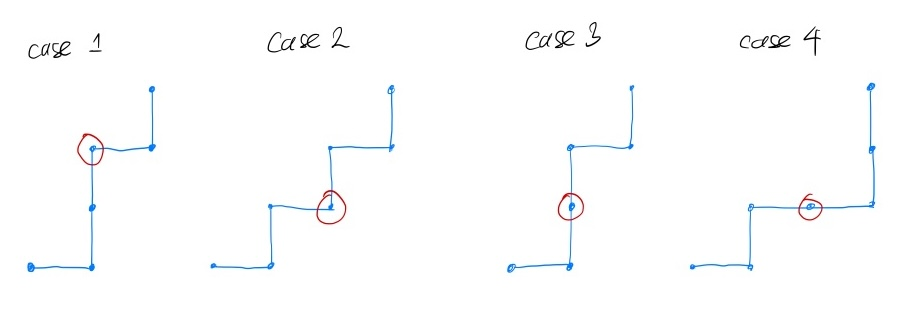
\includegraphics[width=0.7\textwidth]{staircase.jpg}
\caption{4 staircases, note that if removing vertex is at the beginning or the end of staircase, it falls into these 4 cases by shifting indices of $\gamma, \Delta^p, \Delta^q$ by $2$ since shifting by $2$ does not change the sign of boundary map of singular simplex and sign of Eilenberg-Zilber map}
\label{fig_staircase}
\end{figure}

\subsubsection{Case 1, 2}

There is a bijection of $(\gamma, i)$ of case 1 and $(\gamma', i')$ of case 2 ($i = i'$) such that the composition $\gamma d^i$ and $\gamma' d^{i'}$ result in the same map $\Delta^{n-1} \to \Delta^p \times \Delta^q$. Moreover, as the area under the staircase of $\gamma$ and $\gamma'$ differ by one unit square, $A(\gamma) = - A(\gamma')$. Hence, all pairs $(\gamma, i)$, $(\gamma', i')$ cancel out.

\begin{center}
\begin{tikzcd}
\Delta^{n-1} \arrow[r, "d^i"] \arrow[rr, "\gamma d^i"', bend right] & \Delta^n \arrow[r, "\gamma"] & \Delta^p \times \Delta^q
\end{tikzcd}
\end{center}

\subsubsection{Case 4}

Let the removing vertex be $l_i = (p_i, q_i)$. Note that, $q_{i-1} = q_i = q_{i+1}$, then $(l_{i-1}, l_i, l_{i+1})$ is a triangle on the projection of $\Delta^p \times \Delta^q$ on the subspace $q_\bullet = q_i$. By removing $l_i$, $(x_p \times y_q) \gamma d^i$ corresponds to one of the map in $EZ(\partial x_p \otimes y_q)$, specifically

\begin{align*}
    EZ(\partial x_p \otimes y_q)
    &= \sum_{\gamma_1 \in (p-1, q)} (-1)^{A(\gamma_1)} (\partial x_p \times y_q) \gamma_1 \\
    &= \sum_{\gamma_1 \in (p-1, q)} (-1)^{A(\gamma_1)} \tuple*{\tuple*{\sum_{j=0}^p (-1)^j x_p d^j} \times y_q} \gamma_1 \\
    &= \sum_{\gamma_1 \in (p-1, q)} \sum_{j=1}^p (-1)^{A(\gamma_1)} (-1)^j (x_p \times x_q) (d^j \times 1) \gamma_1
\end{align*}

\begin{center}
\begin{tikzcd}
                                                                                      & \Delta^{p-1} \arrow[r, "d^j"]                          & \Delta^p                 \\
\Delta^{n-1} \arrow[r, "\gamma_1"] \arrow[rr, "(d^j \times 1) \gamma_1"', bend right] & \Delta^{p-1} \times \Delta^q \arrow[r, "d^j \times 1"] & \Delta^p \times \Delta^q
\end{tikzcd}
\end{center}

We will construct a bijection between case 3 and $EZ(\partial x_p \otimes y_q)$. The equality holds if we pick $j = p_i$ and $\gamma_1$ is $\gamma$ with $l_i$ removed.

$$
    (-1)^i (-1)^{A(\gamma)} (x_p \times x_q) \gamma d^i = (-1)^{A(\gamma_1)} (-1)^j (x_p \times x_q) (d^j \times 1) \gamma_1
$$

By removing $l_i = (p_i, q_i)$, the map $\gamma d^i$ factors through $(d^j \times 1) \gamma_1$, that is, $(x_p \times x_q) \gamma d^i = (x_p \times x_q) (d^j \times 1) \gamma_1$. Furthermore, we have two equalities $i = p_i + q_i$ and $A(\gamma) = q_i A(\gamma_1)$, then $(-1)^i (-1)^{A(\gamma)} = (-1)^{A(\gamma_1)} (-1)^j$. Note that, this is indeed a bijection since the only case the map $\gamma d^i$ factors through $(d^j \times 1) \gamma_1$ is when $p_i$ appears once in the sequence $(l_1, l_2, ..., l_n)$. Figure \ref{fig_staircase_removed} is an illustration when $p=3, q=2, q_i = 1$

\begin{figure}[h]
\centering
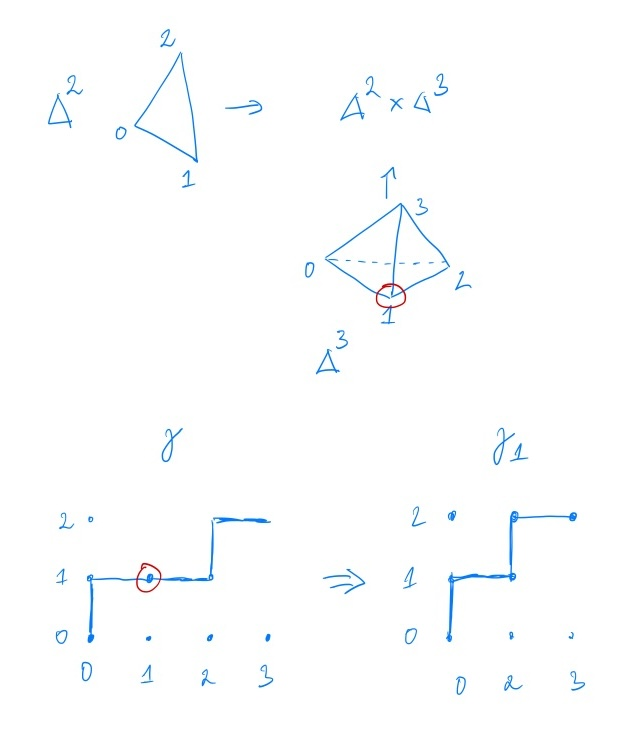
\includegraphics[width=0.5\textwidth]{staircase_removed.jpg}
\caption{staircase removed}
\label{fig_staircase_removed}
\end{figure}

\subsubsection{Case 3}

Case 3 is similar to case 4, the bijection is on $EZ(x_p \otimes \partial y_q)$


\section{Problem 5}

Let $K$ denote the Klein bottle, obtained by gluing two Möbius strips together along their boundaries. Compute the graded abelian group $H_*(K \times K \times K)$

\subsection{Homology of $K$}

\begin{figure}[h]
\centering
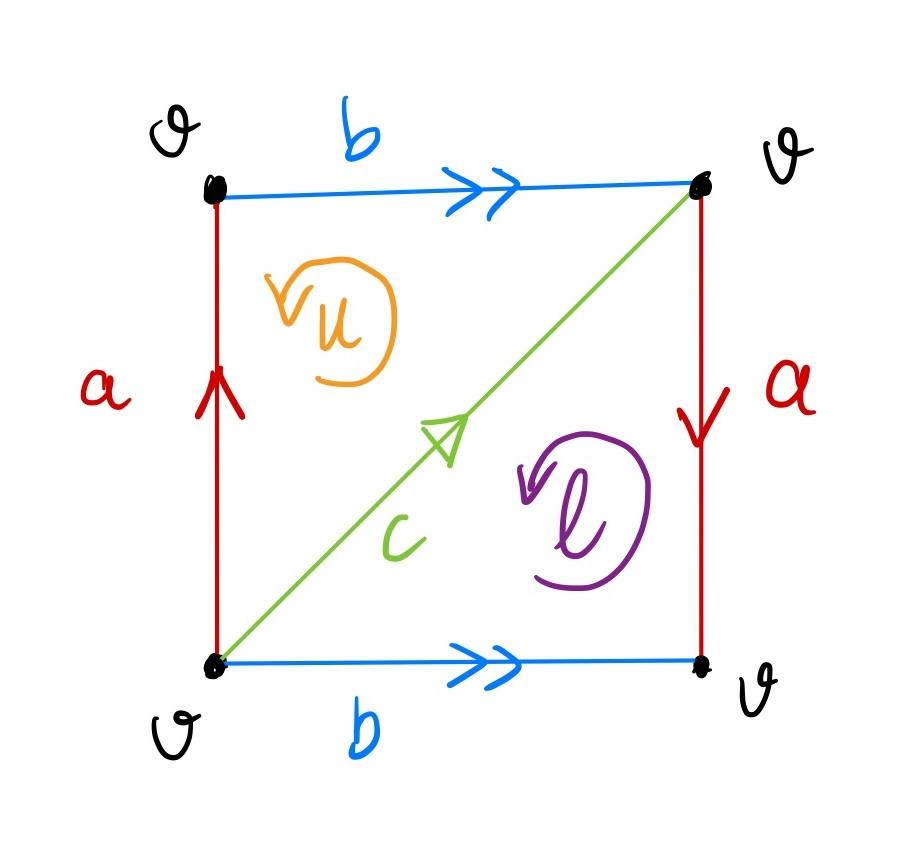
\includegraphics[width=0.3\textwidth]{klein.jpg}
\caption{Klein bottle}
\label{fig_klein}
\end{figure}

Denote the $\Delta$-complex diagram as in Figure \ref{fig_klein},

\begin{center}
\begin{tikzcd}
dim: & 0            & 1                            & 2                            & 3           & ... \\
0    & \Z \arrow[l] & 3\Z \arrow[l, "\partial_1"'] & 2\Z \arrow[l, "\partial_2"'] & 0 \arrow[l] & ...
\end{tikzcd}
\end{center}

Then, the map $\partial_1$ and $\partial_2$ are defined as follows

\begin{align*}
    \partial_1: C_1 &\to C_0 \\
    a &\mapsto 0 \\
    b &\mapsto 0 \\
    c &\mapsto 0 \\
    \partial_2: C_2 &\to C_1 \\
    u &\mapsto -a -b +c \\
    l &\mapsto -a +b -c
\end{align*}

As $\partial_1 = 0$, then

$$
    H_0(K) = \Z
$$

Let change of basis as follows

\begin{align*}
    a' = -a + b - c \\
    b' = b - c \\
    c' = c \\
\end{align*}

as such $\inner{a', b', c'} = \inner{a, b, c}$. Then 
\begin{align*}
    \partial_2: C_2 &\to C_1 \\
    u &\mapsto a' - 2b' \\
    l &\mapsto a'
\end{align*}

For any $2$-chain of the form $pu + ql$ where $p, q \in \Z$, then 

$$
    \partial_2(pu + ql) = (p+q)a' - 2pb'
$$

$\partial_2(pu + ql) = 0$ if and only if $p = q = 0$. That is, $\ker \partial_2 = 0$, then 

$$
    H_2(K) = 0 
$$

Moreover, by setting $p = 0$ and $p = -q$, 

$$
    \im \partial_2 = \inner{a', 2b'}
$$

Then,

$$
    H_1(K) = \frac{\ker \partial_1}{\im \partial_2} = \frac{\inner{a', b', c'}}{\inner{a', 2b'}} = \Z \oplus \Z / 2
$$



\subsection{Some prerequisites}

\begin{proposition}
    The set of abelian groups, $\oplus$ and $\otimes$ form a commutative semiring with additive identity $0$ and multiplicative identity $\Z$
\end{proposition}

In the following, let $A, B, C$ be abelian groups, $n \in \N$
\begin{itemize}
    \item $a := \Z, b := \Z / 2$
    \item $A + B := A \oplus B$
    \item $nA := A \oplus A \oplus ... \oplus A$ ($n$ times)
    \item $A^n := A \otimes A \otimes ... \otimes A$ ($n$ times)
    \item $AB := A \otimes B$
    \item $AB + C := (AB) + C$ (order of operations)
    \item $(A + B) C = AC + BC, C (A + B) = CA + CB$ (left/right distributivity)
    \item $n(AB) = (nA)B$ write $nAB$
    \item $A + B = B + A, AB = BA$ (commutativity)
    \item $aA = Aa = A$
    \item $b^2 = b$ ($\Z/m \otimes \Z/n = \Z/gcd(m, n)$)
    \item $T(A, B) := \Tor^\Z_1(A, B)$
    \item $T(a, A) = T(A, a) = 0$ ($a = \Z$ is free over $\Z$)
    \item $T(b, b) = \Tor^\Z_1(\Z/2, \Z/2) = \ker (2: \Z/2 \to \Z/2) = \Z/2 = b$
    \item $T(A, B) = T(B, A)$ ($\Tor$ symmetric)
    \item $T(A + B, C) = T(A, C) + T(B, C)$ ($\Tor$ commutes with direct product)
    \item $T(nA, B) = nT(A, B)$
\end{itemize}

\begin{theorem}[Künneth theorem]
    If $R$ is an PID, $C_\bullet(X), C_\bullet(Y)$ are degree-wise free then the short exact sequence below is natural and splits
\begin{center}
\begin{tikzcd}
0 \arrow[r] & \bigoplus_{p+q=n} H_p(X; R) \otimes_R H_q(Y; R) \arrow[r] & H_n(X \times Y; R) \arrow[r] & \bigoplus_{p+q=n-1} \Tor^R_1(H_p(X; R), H_q(Y; R))\arrow[r] & 0
\end{tikzcd}
\end{center}
\end{theorem}

Hence,

$$
    H_n(X \times Y; R) = \tuple*{\bigoplus_{p+q=n} H_p(X; R) \otimes_R H_q(Y; R)} \oplus \tuple*{\bigoplus_{p+q=n-1} \Tor^R_1(H_p(X; R), H_q(Y; R))}
$$

Homology of $K$:

\begin{align*}
    H_0(K) &= a \\
    H_1(K) &= a + b \\
    H_q(K) &= 0 &\text{$3 \leq q$}
\end{align*}

\subsection{Homology of $K^2 = K \times K$}

\begin{align*}
    H_0(K^2)
    &= H_0(K) H_0(K) \\
    &= aa = a \\
    H_1(K^2)
    &= H_1(K) H_0(K) + H_0(K) H_1(K) + T(H_0(K), H_0(K)) \\
    &= H_1(K) + H_1(K) &\text{($H_0(K) = a$)} \\
    &= 2a + 2b \\
    H_2(K^2)
    &= H_1(K) H_1(K) + T(H_1(K), H_0(K)) + T(H_0(K), H_1(K)) \\
    &= H_1(K) H_1(K) &\text{($H_0(K) = a$)} \\
    &= (a + b) (a + b) \\
    &= a^2 + ba + ab + b^2 \\
    &= a + 2b + b^2 \\
    &= a + 3b \\
    H_3(K^2)
    &= T(H_1(K), H_1(K)) \\
    &= T(a + b, a + b) \\
    &= T(a, a) + T(a, b) + T(b, a) + T(b, b) \\
    &= T(b, b) \\
    &= b
\end{align*}

In summary

\begin{align*}
    H_0(K^2)
    &= a \\
    H_1(K^2)
    &= 2a + 2b \\
    H_2(K^2)
    &= a + 3b \\
    H_3(K^2)
    &= b \\
    H_q(K^2) &= 0 &\text{for all $4 \leq q$}
\end{align*}

\subsection{Homology of $K^3 = K \times K \times K$}

\begin{align*}
    H_0(K^3)
    &= H_0(K^2) \otimes H_0(K) \\
    &= aa = a \\
    H_1(K^3)
    &= H_1(K^2) H_0(K) + H_0(K^2) H_1(K) + T(H_0(K^2), H_0(K)) \\
    &= H_1(K^2) + H_1(K) &\text{($H_0(K) = H_0(K^2) = a$)}\\
    &= 2a + 2b + a + b \\
    &= 3a + 3b \\
    H_2(K^3)
    &= H_2(K^2) H_0(K) + H_1(K^2) H_1(K) \\ &+ T(H_1(K^2), H_0(K)) + T(H_0(K^2), H_1(K)) \\
    &= H_2(K^2) + H_1(K^2) H_1(K) &\text{($H_0(K) = H_0(K^2) = a$)} \\
    &= a + 3b + (2a + 2b)(a + b) \\
    &= a + 3b + 2a(a + b) + 2b(a + b) \\
    &= a + 3b + 2a^2 + 2ab + 2ba + 2b^2 \\
    &= a + 3b + 2a + 2b + 2b + 2b \\
    &= 3a + 9b \\
    H_3(K^3)
    &= H_3(K^2) H_0(K) + H_2(K^2) H_1(K) \\&+ T(H_2(K^2), H_0(K)) + T(H_1(K^2), H_1(K)) + T(H_0(K^2), H_2(K)) \\
    &= H_3(K^2) + H_2(K^2) H_1(K) + T(H_1(K^2), H_1(K)) &\text{($H_0(K) = H_0(K^2) = a$)} \\
    &= b + (a + 3b)(a + b) + T(2a + 2b, a + b) \\
    &= b + a^2 + ab + 3ba + 3b^2 + 2T(a, a) + 2T(a, b) + 2T(b, a) + 2T(b, b) \\
    &= b + a + b + 3b + 3b + b \\
    &= a + 9b \\
    H_4(K^3)
    &= H_3(K^2) H_1(K) + T(H_3(K^2), H_0(K)) + T(H_2(K^2), H_1(K)) \\
    &= H_3(K^2) H_1(K) + T(H_2(K^2), H_1(K)) &\text{($H_0(K) = a$)} \\
    &= b (a + b) + T(a + 3b, a + b) \\
    &= ba + b^2 + T(a, a) + T(a, b) + 3T(b, a) + 3T(b, b) \\
    &= b + b + 3b \\
    &= 5b \\
    H_5(K^3)
    &= T(H_3(K^2), H_1(K)) \\
    &= T(b, a + b) \\
    &= T(b, a) + T(b, b) \\
    &= b
\end{align*}

In summary,

\begin{align*}
    H_0(K^3) &= a = \Z \\
    H_1(K^3) &= 3a + 3b = 3 \Z \oplus 3 (\Z/2) \\
    H_2(K^3) &= 3a + 9b = 3 \Z \oplus 9 (\Z/2) \\
    H_3(K^3) &= a + 9b = \Z \oplus 9 (\Z/2) \\
    H_4(K^3) &= 5b = 5 (\Z / 2) \\
    H_5(K^3) &= b = \Z / 2 \\
    H_q(K^3) &= 0 &\text{for all $6 \leq q$} \\
\end{align*}


\end{document}
